\documentclass[10pt,twocolumn,a4paper]{article}

% -------------------------------------------------
% Language and encoding
% -------------------------------------------------
\usepackage[T1]{fontenc}
\usepackage{lmodern}
\usepackage[english]{babel}

% -------------------------------------------------
% Document format
% -------------------------------------------------
\usepackage[
    top=1.8cm,
    bottom=1.8cm,
    left=1.8cm,
    right=1.8cm,
    columnsep=0.7cm
]{geometry}

\usepackage{microtype}
\usepackage{parskip}

% -------------------------------------------------
% Mathematics
% -------------------------------------------------
\usepackage{amsmath}
\usepackage{amssymb}
\usepackage{bm}

% -------------------------------------------------
% Figures and tables
% -------------------------------------------------
\usepackage{graphicx}
\usepackage{booktabs}
\usepackage{siunitx}
\usepackage{subcaption}

% -------------------------------------------------
% Links and references
% -------------------------------------------------
\usepackage[hidelinks]{hyperref}

% Image folder for later figures
\graphicspath{{images/}}

% -------------------------------------------------
% Document information
% -------------------------------------------------
\title{
    \textbf{Integrated Mobile Robot Navigation\\
    with Reactive Obstacle Avoidance\\
    and Filtered Range Sensors}
}

\author{
    Julio Quejido Barrera\\
    Humanoide Robotik\\
    Julio's Laboratories
}

\date{\today}

% =================================================
\begin{document}
% =================================================

\maketitle

\begin{abstract}
This project integrates goal-seeking control, finite range-sensor rays,
geometric obstacle detection, reactive obstacle avoidance, Gaussian
measurement noise, and exponential sensor filtering in a single mobile
robot simulation. In free space, the robot follows a goal using a
proportional angular controller and a distance-dependent linear-speed
law with saturation. Three range sensors, oriented to the left, right,
and front of the robot, test finite rays against circular obstacles.
When an obstacle is detected, a priority-based reactive controller
temporarily replaces the goal-seeking behavior. The ideal ray--circle
intersection distance is then treated as a sensor measurement, corrupted
with additive Gaussian noise, and smoothed using a first-order
exponential moving-average filter. The resulting system represents an
integrated sensing--decision--motion pipeline in which continuous
feedback control is combined with discrete reactive rules and basic
signal processing.
\end{abstract}

\section{Introduction}

A mobile robot that moves toward a target must continuously solve three
related problems. First, it must calculate how fast to move and how much
to rotate in order to approach the goal. Second, it must perceive nearby
obstacles and determine whether its current motion is safe. Third, it
must deal with imperfect sensor measurements, because real distance
sensors do not return exact geometric values.

The present project combines these problems in one simulation. The
vector and angular operations developed in the previous projects are
reused to calculate the current distance and normalized angular error.
These quantities are now converted into linear and angular velocities.
At the same time, three finite sensor rays are generated from the robot
pose and tested against a set of circular obstacles. The closest valid
intersection detected by each sensor is converted into a binary
left--right--front perception state.

The navigation behavior is selected by priority. If no sensor detects
an obstacle, the robot follows the goal with proportional control. If an
obstacle is detected, the goal controller is temporarily replaced by a
reactive avoidance rule. Finally, Gaussian noise and exponential
smoothing are introduced so that the control decision is based on a
filtered measurement rather than on an ideal intersection distance.
This extends the simulation from pure geometry to an integrated model
of control, perception, uncertainty, and filtering.

\section{Theoretical Background}

\subsection{Distance to the Goal and Stopping Criterion}

Let the robot position at simulation step $k$ be
$\mathbf{p}_k=[x_k,y_k]^T$ and let the fixed goal position be
$\mathbf{p}_G$. The Euclidean distance, already introduced in the first
project, is reused as the main translational feedback variable:

\begin{equation}
    d_k = \left\|\mathbf{p}_G-\mathbf{p}_k\right\|.
    \label{eq:goal_distance}
\end{equation}

The simulation terminates when the robot enters a circular tolerance
region around the goal:

\begin{equation}
    d_k < d_{\mathrm{tol}},
    \qquad
    d_{\mathrm{tol}}=0.01.
    \label{eq:stopping_condition}
\end{equation}

The distance is therefore not rederived here as a geometric concept; it
is used as a feedback signal, a stopping condition, and an input to the
linear-speed controller.

\subsection{Normalized Angular Error}

The robot-to-goal vector is

\[
    \mathbf{v}_{G,k}=\mathbf{p}_G-\mathbf{p}_k.
\]

Its absolute direction is calculated with the two-argument arctangent
and converted to degrees:

\begin{equation}
    \theta_{G,k}^{\circ}
    =
    \frac{180^{\circ}}{\pi}
    \operatorname{atan2}(v_{G,y,k},v_{G,x,k}).
    \label{eq:goal_angle_deg}
\end{equation}

The angular error reused by the controller is the shortest signed
difference between the goal direction and the current robot orientation:

\begin{equation}
    e_{\theta,k}
    =
    \left(
    \theta_{G,k}^{\circ}-\theta_k^{\circ}+180^{\circ}
    \right)
    \bmod 360^{\circ}
    -180^{\circ}.
    \label{eq:angle_error_deg}
\end{equation}

Consequently,

\[
    -180^{\circ}
    \leq e_{\theta,k}
    <180^{\circ}.
\]

Angle normalization was developed in the previous project. Its new role
here is to provide a continuous control error whose sign specifies the
shortest turning direction and whose magnitude specifies the required
orientation correction.

\subsection{Angular Proportional Controller}

In free space, the angular velocity is generated by a proportional
controller:

\begin{equation}
    \omega_k = K_{\theta}e_{\theta,k}.
    \label{eq:p_angular_controller}
\end{equation}

The implemented angular gain is

\[
    K_{\theta}=0.5.
\]

Because $e_{\theta,k}$ is represented in degrees, $\omega_k$ is treated
as a rotational rate in degrees per unit time. A large orientation error
produces a large turning command, while a small error produces a slower
correction. When the robot is aligned with the goal,
$e_{\theta,k}=0$ and the proportional command becomes $\omega_k=0$.

This equation marks the transition from angular analysis to closed-loop
motion control. In the previous project, the error only indicated left,
right, or straight. Here, the same error directly determines the
continuous turning rate.

\subsection{Linear-Speed Control and Saturation}

When the path is free, the desired linear speed is proportional to the
distance from the goal:

\begin{equation}
    v_k^{\mathrm{raw}}=K_v d_k.
    \label{eq:raw_linear_speed}
\end{equation}

A maximum-speed limit is applied to avoid commanding a value above the
allowed motor speed:

\begin{equation}
    v_k
    =
    \min\left(K_vd_k,\,v_{\max}\right).
    \label{eq:saturated_linear_speed}
\end{equation}

Equivalently,

\begin{equation}
    v_k=
    \begin{cases}
        K_vd_k, & K_vd_k<v_{\max},\\[1mm]
        v_{\max}, & K_vd_k\geq v_{\max}.
    \end{cases}
    \label{eq:piecewise_speed}
\end{equation}

The initial values used by the simulation are

\[
    K_v=0.5,
    \qquad
    v_{\max}=1.0.
\]

Far from the goal, the command reaches the saturation limit. As the
robot approaches the target, the proportional term decreases and the
robot slows down progressively.

\subsection{Near-Goal Parameter Adjustment}

Inside a distance of one unit from the goal, the simulation reduces both
the linear gain and the sensor range:

\begin{equation}
    K_v(d_k)=
    \begin{cases}
        0.5, & d_k\geq 1,\\
        0.1, & d_k<1,
    \end{cases}
    \label{eq:gain_schedule}
\end{equation}

and

\begin{equation}
    R_s(d_k)=
    \begin{cases}
        0.5, & d_k\geq 1,\\
        0.3, & d_k<1.
    \end{cases}
    \label{eq:range_schedule}
\end{equation}

This is a simple form of parameter scheduling. The smaller linear gain
reduces the approach speed near the target, while the shorter sensor
range makes the local avoidance region more compact. In the implemented
simulation these values are assigned once the condition $d_k<1$ is
satisfied and are not explicitly reset later.

\subsection{Discrete Robot Motion Model}

The orientation angle is converted into a unit heading vector. Since the
stored orientation is expressed in degrees, it is first converted to
radians:

\begin{equation}
    \theta_k^{\mathrm{rad}}
    =
    \frac{\pi}{180^{\circ}}\theta_k^{\circ}.
    \label{eq:deg_to_rad}
\end{equation}

The corresponding heading is

\begin{equation}
    \mathbf{h}_k
    =
    \begin{bmatrix}
        \cos\theta_k^{\mathrm{rad}}\\
        \sin\theta_k^{\mathrm{rad}}
    \end{bmatrix}.
    \label{eq:heading_vector}
\end{equation}

The orientation update is

\begin{equation}
    \theta_{k+1}^{\circ}
    =
    \theta_k^{\circ}+\omega_k\Delta t.
    \label{eq:orientation_update}
\end{equation}

After updating the orientation, the new heading is used to advance the
position:

\begin{equation}
    \mathbf{p}_{k+1}
    =
    \mathbf{p}_k
    +v_k\mathbf{h}_{k+1}\Delta t.
    \label{eq:position_update}
\end{equation}

In coordinate form,

\begin{align}
    x_{k+1}
    &=x_k+v_k\cos\theta_{k+1}^{\mathrm{rad}}\Delta t,
    \\n    y_{k+1}
    &=y_k+v_k\sin\theta_{k+1}^{\mathrm{rad}}\Delta t.
    \label{eq:coordinate_update}
\end{align}

The time step is $\Delta t=0.01$. This discrete update is a simple
unicycle-like kinematic model in which the control inputs are the linear
speed $v_k$ and angular speed $\omega_k$.

\subsection{Finite Range-Sensor Rays}

The robot carries three sensors with fixed relative orientations:

\begin{equation}
    \beta_L=45^{\circ},
    \qquad
    \beta_R=-45^{\circ},
    \qquad
    \beta_F=0^{\circ}.
    \label{eq:sensor_relative_angles}
\end{equation}

For sensor $s\in\{L,R,F\}$, the global sensor angle is obtained by
adding the relative sensor orientation to the robot orientation:

\begin{equation}
    \phi_{s,k}=\theta_k+\beta_s.
    \label{eq:sensor_global_angle}
\end{equation}

The sensor direction is the unit vector

\begin{equation}
    \mathbf{u}_{s,k}
    =
    \begin{bmatrix}
        \cos\phi_{s,k}^{\mathrm{rad}}\\
        \sin\phi_{s,k}^{\mathrm{rad}}
    \end{bmatrix}.
    \label{eq:sensor_direction}
\end{equation}

A finite sensor ray is represented parametrically as

\begin{equation}
    \mathbf{r}_{s,k}(t)
    =
    \mathbf{p}_k+t\mathbf{u}_{s,k},
    \qquad
    0\leq t\leq R_s.
    \label{eq:sensor_ray}
\end{equation}

Its endpoint is therefore

\begin{equation}
    \mathbf{p}^{\mathrm{end}}_{s,k}
    =
    \mathbf{p}_k+R_s\mathbf{u}_{s,k}.
    \label{eq:sensor_endpoint}
\end{equation}

Unlike an infinite mathematical line, this model only detects objects
inside the interval from the robot position to the maximum range $R_s$.

\subsection{Circular Obstacle Model}

Each obstacle $j$ is represented by a center
$\mathbf{c}_j=[c_{x,j},c_{y,j}]^T$ and a radius $r_j$. Its boundary is

\begin{equation}
    \left\|\mathbf{p}-\mathbf{c}_j\right\|=r_j.
    \label{eq:circular_obstacle}
\end{equation}

For a given robot position, the vector from the robot to the obstacle
center is

\begin{equation}
    \mathbf{q}_{j,k}=\mathbf{c}_j-\mathbf{p}_k.
    \label{eq:robot_to_obstacle}
\end{equation}

The simulation tests every sensor ray against every circular obstacle.
The geometric procedure first determines whether an intersection is
possible and then calculates the first point at which the ray enters the
circle.

\subsection{Projection onto the Sensor Direction}

The scalar projection of the obstacle-center vector onto the unit sensor
direction is

\begin{equation}
    \lambda_{s,j,k}
    =
    \mathbf{q}_{j,k}\cdot\mathbf{u}_{s,k}.
    \label{eq:projection}
\end{equation}

Because $\mathbf{u}_{s,k}$ is normalized, $\lambda_{s,j,k}$ is the
longitudinal distance from the robot to the orthogonal projection of the
obstacle center on the sensor line.

Before performing the complete intersection calculation, the obstacle
is rejected when its projected interval does not overlap the finite ray:

\begin{equation}
    \lambda_{s,j,k}+r_j<0
    \quad\text{or}\quad
    \lambda_{s,j,k}-r_j>R_s.
    \label{eq:range_rejection}
\end{equation}

This inexpensive test excludes circles located completely behind the
sensor or completely beyond its maximum range.

\subsection{Closest Point and Perpendicular Distance}

The point on the sensor line closest to the obstacle center is

\begin{equation}
    \mathbf{p}^{\mathrm{close}}_{s,j,k}
    =
    \mathbf{p}_k
    +\lambda_{s,j,k}\mathbf{u}_{s,k}.
    \label{eq:closest_point}
\end{equation}

The perpendicular distance from the obstacle center to the sensor line
is

\begin{equation}
    d^{\perp}_{s,j,k}
    =
    \left\|
    \mathbf{c}_j-\mathbf{p}^{\mathrm{close}}_{s,j,k}
    \right\|.
    \label{eq:distance_to_ray}
\end{equation}

An intersection with the infinite sensor line is possible only if

\begin{equation}
    d^{\perp}_{s,j,k}\leq r_j.
    \label{eq:line_circle_condition}
\end{equation}

If $d^{\perp}_{s,j,k}>r_j$, the ray passes outside the circle and the
obstacle is ignored.

\subsection{Ray--Circle Intersection Distance}

When the line intersects the circle, the projection, radius, and
perpendicular distance form a right triangle. The longitudinal offset
from the projected center to either intersection is

\begin{equation}
    \delta_{s,j,k}
    =
    \sqrt{r_j^2-\left(d^{\perp}_{s,j,k}\right)^2}.
    \label{eq:intersection_offset}
\end{equation}

The two line--circle intersection parameters are

\begin{equation}
    t^{\mathrm{near}}_{s,j,k}
    =
    \lambda_{s,j,k}-\delta_{s,j,k},
    \label{eq:near_intersection}
\end{equation}

and

\begin{equation}
    t^{\mathrm{far}}_{s,j,k}
    =
    \lambda_{s,j,k}+\delta_{s,j,k}.
    \label{eq:far_intersection}
\end{equation}

The simulation uses the near intersection because it corresponds to the
first obstacle surface reached by the ray. A geometric hit is accepted
only if

\begin{equation}
    0\leq t^{\mathrm{near}}_{s,j,k}\leq R_s.
    \label{eq:finite_ray_condition}
\end{equation}

Without measurement noise, the ideal hit point would be

\begin{equation}
    \mathbf{p}^{\mathrm{hit}}_{s,j,k}
    =
    \mathbf{p}_k
    +t^{\mathrm{near}}_{s,j,k}\mathbf{u}_{s,k}.
    \label{eq:ideal_hit_point}
\end{equation}

\subsection{Nearest Detection per Sensor}

A single sensor ray may intersect more than one obstacle. Let
$\mathcal{I}_{s,k}$ denote the set of valid detected obstacles for sensor
$s$ at step $k$. The selected obstacle is the one with the smallest
accepted measurement distance:

\begin{equation}
    j_{s,k}^{*}
    =
    \underset{j\in\mathcal{I}_{s,k}}{\operatorname{arg\,min}}
    \;d^{\mathrm{meas}}_{s,j,k}.
    \label{eq:nearest_detection}
\end{equation}

Each sensor therefore returns either no detection or one record
containing the nearest valid obstacle, its measured distance, the hit
point, and the associated geometric closest point.

\subsection{Binary Sensor State}

The three selected sensor outputs are converted into binary states:

\begin{equation}
    D_L,D_R,D_F\in\{0,1\}.
    \label{eq:binary_sensor_states}
\end{equation}

A value of one means that the corresponding left, right, or front sensor
contains a valid detection. These binary variables remove the detailed
geometric information from the final avoidance decision and allow the
robot to apply a compact rule-based controller.

\subsection{Reactive Obstacle Avoidance}

The avoidance behavior directly assigns linear and angular velocities
from the binary sensor state. The implemented rules are summarized in
Table~\ref{tab:reactive_rules}. Positive angular velocity represents a
left turn, while negative angular velocity represents a right turn.

\begin{table}[htbp]
\centering
\caption{Priority-Ordered Reactive Avoidance Rules.}
\label{tab:reactive_rules}
\small
\resizebox{\columnwidth}{!}{%
\begin{tabular}{clccl}
\toprule
\textbf{Priority} & \textbf{Detection} & $v_k$ & $\omega_k$ & \textbf{Response} \\
\midrule
1 & $D_L\land D_F$ & $0.25$ & $-90$ & turn right \\
2 & $D_R\land D_F$ & $0.25$ & $+90$ & turn left \\
3 & $D_R\land D_L$ & $0.10$ & $0$ & move slowly forward \\
4 & $D_F$ & $0.10$ & $+50$ & turn left \\
5 & $D_L$ & $0.50$ & $-70$ & turn right \\
6 & $D_R$ & $0.50$ & $+70$ & turn left \\
\bottomrule
\end{tabular}%
}
\end{table}

The ordering is part of the controller. The conditions are evaluated
sequentially, and only the first valid rule is executed. For example, if
all three sensors detect simultaneously, the first condition
$D_L\land D_F$ is satisfied and the robot applies the right-turn rule.
The controller is reactive because it maps the current sensor state
directly to an action without predicting future motion.

\subsection{Behavior Arbitration}

The system combines two behaviors: obstacle avoidance and goal seeking.
Let the control vector be

\begin{equation}
    \mathbf{u}_k=
    \begin{bmatrix}
        v_k\\
        \omega_k
    \end{bmatrix}.
    \label{eq:control_vector}
\end{equation}

The arbitration rule is

\begin{equation}
    \mathbf{u}_k=
    \begin{cases}
        \mathbf{u}^{\mathrm{avoid}}_k,
        & D_L\lor D_R\lor D_F,\\[1mm]
        \mathbf{u}^{\mathrm{goal}}_k,
        & \neg(D_L\lor D_R\lor D_F),
    \end{cases}
    \label{eq:behavior_arbitration}
\end{equation}

where the free-space goal controller is

\begin{equation}
    \mathbf{u}^{\mathrm{goal}}_k
    =
    \begin{bmatrix}
        \min(K_vd_k,v_{\max})\\
        K_{\theta}e_{\theta,k}
    \end{bmatrix}.
    \label{eq:goal_control_vector}
\end{equation}

Obstacle avoidance has strict priority over goal seeking. The two
commands are not averaged or blended. A detection switches the system
to the reactive mode; when all sensors are free, the proportional goal
controller becomes active again. The complete system is therefore a
simple hybrid or switched controller that combines discrete decisions
with continuous robot motion.

\subsection{Additive Gaussian Sensor Noise}

The geometric near-intersection distance is treated as the ideal sensor
value:

\begin{equation}
    d^{\mathrm{true}}_{s,j,k}
    =
    t^{\mathrm{near}}_{s,j,k}.
    \label{eq:true_sensor_distance}
\end{equation}

A noisy measurement is generated using an additive Gaussian model:

\begin{equation}
    z_n
    =
    d^{\mathrm{true}}_{s,j,k}+\eta_n,
    \label{eq:noisy_measurement}
\end{equation}

with

\begin{equation}
    \eta_n\sim\mathcal{N}(0,\sigma^2).
    \label{eq:gaussian_noise}
\end{equation}

The probability density of the noise is

\begin{equation}
    p(\eta)
    =
    \frac{1}{\sigma\sqrt{2\pi}}
    \exp\left(-\frac{\eta^2}{2\sigma^2}\right).
    \label{eq:gaussian_density}
\end{equation}

The simulation uses

\[
    \sigma=0.5.
\]

For zero-mean noise,

\begin{equation}
    \mathbb{E}[z_n]=d^{\mathrm{true}}_{s,j,k},
    \qquad
    \operatorname{Var}(z_n)=\sigma^2.
    \label{eq:measurement_statistics}
\end{equation}

The measurement is therefore unbiased in expectation, although
individual samples may lie above or below the true distance. Since the
initial sensor range is also $0.5$, the selected standard deviation is
large relative to the physical measurement interval and makes filtering
particularly important.

\subsection{Exponential Moving-Average Filter}

For every valid geometric intersection, the simulation generates a
batch of $N=1000$ noisy measurements of the same ideal distance. The
first-order exponential moving-average estimate is initialized by

\begin{equation}
    \hat{d}_0=z_0
    \label{eq:filter_initialization}
\end{equation}

and updated for $n=1,\ldots,999$ according to

\begin{equation}
    \hat{d}_n
    =
    \alpha z_n+(1-\alpha)\hat{d}_{n-1}.
    \label{eq:ema_filter}
\end{equation}

The implemented coefficient is

\[
    \alpha=0.01.
\]

The final value used by the obstacle-detection logic is

\begin{equation}
    d^{\mathrm{meas}}_{s,j,k}=\hat{d}_{999}.
    \label{eq:final_filtered_measurement}
\end{equation}

The hit point is then recalculated from the filtered distance:

\begin{equation}
    \mathbf{p}^{\mathrm{hit}}_{s,j,k}
    =
    \mathbf{p}_k
    +d^{\mathrm{meas}}_{s,j,k}\mathbf{u}_{s,k}.
    \label{eq:filtered_hit_point}
\end{equation}

After filtering, the measurement must again satisfy

\begin{equation}
    0\leq d^{\mathrm{meas}}_{s,j,k}\leq R_s.
    \label{eq:filtered_range_validation}
\end{equation}

Consequently, a geometric intersection can be rejected if the final
filtered measurement lies outside the valid range.

\subsection{Influence of the Filter Coefficient}

The coefficient $\alpha$ determines the balance between the new noisy
measurement and the previous filtered estimate. When $\alpha$ is small,
the filter gives most of the weight to its previous output:

\[
    \alpha \rightarrow 0
    \quad\Rightarrow\quad
    \hat{d}_n \approx \hat{d}_{n-1}.
\]

This produces strong smoothing because rapid variations in the noisy
measurements have only a small influence on the output. However, the
filtered estimate responds more slowly when the measured distance
changes.

When $\alpha$ approaches one,

\[
    \alpha \rightarrow 1
    \quad\Rightarrow\quad
    \hat{d}_n \approx z_n,
\]

the current measurement has a greater influence on the output. The
filter therefore reacts more quickly, but a larger part of the sensor
noise remains in the filtered signal. At the limiting value
$\alpha=1$, no smoothing is performed.

Repeated substitution of Equation~\eqref{eq:ema_filter} gives

\begin{equation}
    \hat{d}_n
    =
    (1-\alpha)^n z_0
    +
    \alpha
    \sum_{j=1}^{n}
    (1-\alpha)^{n-j}z_j.
    \label{eq:ema_expansion}
\end{equation}

Older measurements therefore receive exponentially decreasing weights.
This allows the filter to maintain a memory of previous values without
storing the complete measurement history during the recursive
calculation.

The influence of $\alpha$ was evaluated using two values,
$\alpha=0.01$ and $\alpha=0.6$, while keeping the noise standard
deviation constant at

\[
    \sigma = 0.5.
\]

For $\alpha=0.01$, the recursive equation becomes

\[
    \hat{d}_n
    =
    0.01z_n
    +
    0.99\hat{d}_{n-1}.
\]

Only one percent of the new measurement is introduced at each
iteration, while the previous filtered estimate contributes
ninety-nine percent. Consequently, the output is highly smoothed, but
several measurements are required before it adapts to a change in the
measured distance.

For $\alpha=0.6$, the filter becomes

\[
    \hat{d}_n
    =
    0.6z_n
    +
    0.4\hat{d}_{n-1}.
\]

In this case, the current measurement contributes sixty percent of the
new estimate. The filtered output therefore follows changes much more
rapidly, although the fluctuations produced by the Gaussian noise are
less attenuated.

\begin{figure*}[t]
    \centering

    \begin{subfigure}[t]{0.48\textwidth}
        \centering
        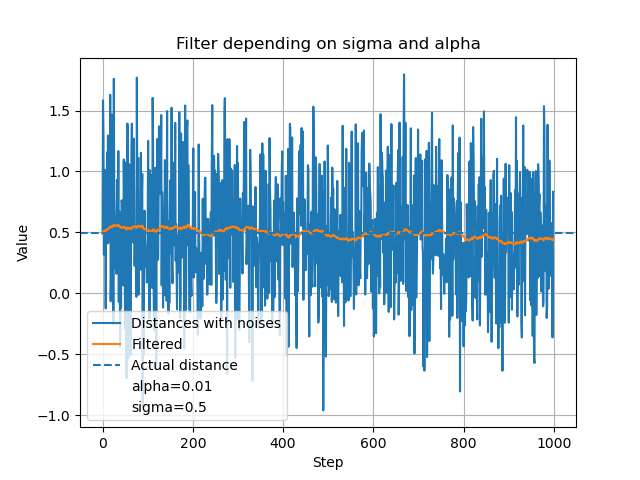
\includegraphics[width=\linewidth]{Filter_1.png}
        \caption{Noisy and filtered sensor measurements for
        $\alpha=0.01$ and $\sigma=0.5$.}
        \label{fig:filter_alpha_001}
    \end{subfigure}
    \hfill
    \begin{subfigure}[t]{0.48\textwidth}
        \centering
        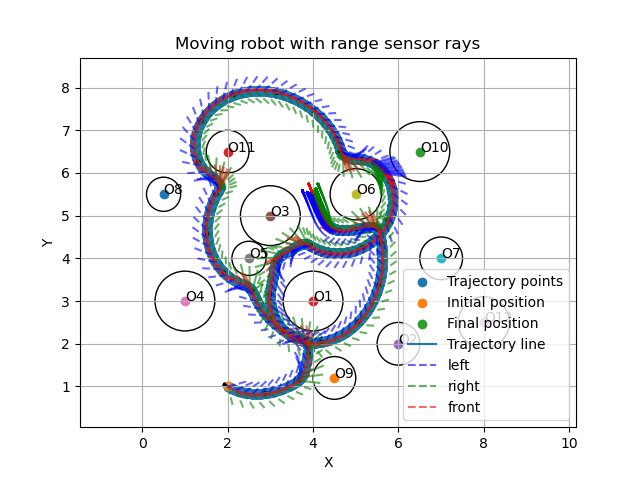
\includegraphics[width=\linewidth]{Figure_1.png}
        \caption{Robot trajectory obtained using
        $\alpha=0.01$.}
        \label{fig:trajectory_alpha_001}
    \end{subfigure}

    \vspace{0.4cm}

    \begin{subfigure}[t]{0.48\textwidth}
        \centering
        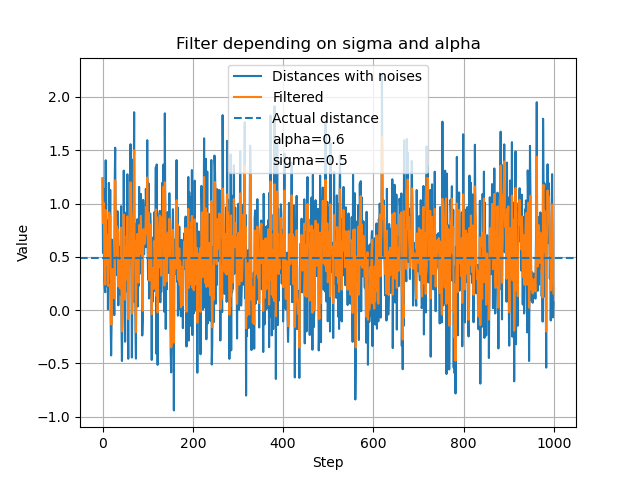
\includegraphics[width=\linewidth]{Filter_2.png}
        \caption{Noisy and filtered sensor measurements for
        $\alpha=0.6$ and $\sigma=0.5$.}
        \label{fig:filter_alpha_06}
    \end{subfigure}
    \hfill
    \begin{subfigure}[t]{0.48\textwidth}
        \centering
        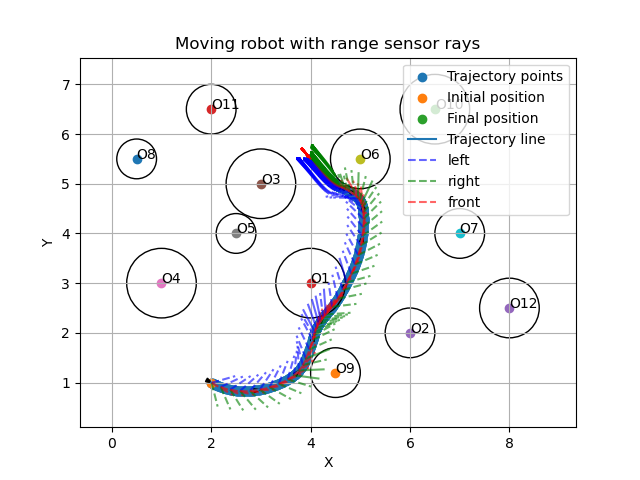
\includegraphics[width=\linewidth]{Figure_2.png}
        \caption{Robot trajectory obtained using
        $\alpha=0.6$.}
        \label{fig:trajectory_alpha_06}
    \end{subfigure}

    \caption{Comparison of the sensor filtering results and the
    corresponding robot trajectories for two exponential-filter
    coefficients. A small value of $\alpha$ produces stronger
    smoothing but a slower response, whereas a larger value produces a
    faster response but retains more measurement noise.}
    \label{fig:alpha_comparison}
\end{figure*}

Figure~\ref{fig:alpha_comparison} shows the effect of the filter
coefficient on the measurements generated for the first obstacle
detection. With $\alpha=0.01$, the filtered signal remains considerably
smoother than the noisy measurements. The strong contribution of the
previous estimate prevents individual noisy samples from causing large
changes in the filter output.

With $\alpha=0.6$, the filtered signal follows the noisy measurements
more closely. This allows it to adapt more rapidly, but the output
contains noticeably larger fluctuations. Therefore, increasing
$\alpha$ improves the response speed at the cost of weaker noise
attenuation.

The trajectory plots show the combined result of goal-seeking control,
range sensing, filtered obstacle detection, and reactive avoidance.
However, the simulated sensor noise is generated randomly. Consequently,
differences between individual trajectories are influenced both by the
selected value of $\alpha$ and by the particular noise samples generated
during each simulation run.

\subsection{Filter Transfer Function and Noise Reduction}

Ignoring initial conditions, the filter relation can be written in the
$z$ domain as

\begin{equation}
    H(z)
    =
    \frac{\hat{D}(z)}{Z(z)}
    =
    \frac{\alpha}
    {1-(1-\alpha)z^{-1}}.
    \label{eq:filter_transfer_function}
\end{equation}

The pole is

\begin{equation}
    z_p=1-\alpha.
    \label{eq:filter_pole}
\end{equation}

For $0<\alpha\leq 1$, the pole lies inside the unit circle and the filter
is stable. Under the assumptions of a constant true distance and
independent white Gaussian noise, the steady-state output variance is

\begin{equation}
    \operatorname{Var}(\hat{d})
    =
    \frac{\alpha}{2-\alpha}\sigma^2.
    \label{eq:filtered_variance}
\end{equation}

For $\alpha=0.01$, the theoretical variance factor is

\[
    \frac{0.01}{2-0.01}\approx 0.00503.
\]

Thus, the selected coefficient strongly reduces the noise variance for
a constant distance, at the cost of a slower transient response.

\section{Integrated Method}

\subsection{Simulation Configuration}

The main simulation parameters are summarized in
Table~\ref{tab:simulation_parameters}. The environment contains twelve
circular obstacles with individually specified centers and radii.

\begin{table}[htbp]
\centering
\caption{Main Simulation Parameters.}
\label{tab:simulation_parameters}
\small
\begin{tabular}{ll}
\toprule
\textbf{Parameter} & \textbf{Value} \\
\midrule
Initial robot position & $[2.0,\,1.0]^T$ \\
Goal position & $[4.0,\,5.5]^T$ \\
Initial orientation & $-30^{\circ}$ \\
Time step $\Delta t$ & $0.01$ \\
Maximum simulation steps & $10000$ \\
Goal tolerance & $0.01$ \\
Initial sensor range & $0.5$ \\
Near-goal sensor range & $0.3$ \\
Angular gain $K_{\theta}$ & $0.5$ \\
Initial linear gain $K_v$ & $0.5$ \\
Near-goal linear gain & $0.1$ \\
Maximum linear speed & $1.0$ \\
Noise standard deviation & $\sigma=0.5$ \\
Filter coefficient & $\alpha=0.01$ \\
Samples per filtered hit & $1000$ \\
\bottomrule
\end{tabular}
\end{table}

\subsection{Sensing--Decision--Motion Cycle}

At every simulation step, the method performs the following sequence:

\begin{enumerate}
    \item Calculate the current distance to the goal and stop if the
    tolerance has been reached.

    \item Apply the near-goal parameter adjustment when $d_k<1$.

    \item Construct the left, right, and front finite sensor rays from
    the current robot pose.

    \item Test every sensor ray against every circular obstacle using
    projection, perpendicular distance, and ray--circle intersection.

    \item For each valid geometric hit, generate a batch of $1000$ noisy
    Gaussian measurements and apply the exponential moving-average filter.

    \item Reject filtered distances outside the finite sensor range and
    retain the closest valid obstacle for each sensor.

    \item Convert the three sensor outputs into the binary variables
    $D_L$, $D_R$, and $D_F$.

    \item If any sensor detects an obstacle, apply the first matching
    reactive rule. Otherwise, calculate $v_k$ and $\omega_k$ with the
    goal-seeking controllers.

    \item Update the robot orientation, recompute its heading, and
    advance the position using the discrete motion model.

    \item Store the trajectory, orientation, speed, angular error,
    distance to the goal, sensor endpoints, and current detections.
\end{enumerate}

This order creates the complete information flow

\[
\begin{aligned}
\text{geometry}
&\rightarrow \text{sensing}
\rightarrow \text{noise}\\
&\rightarrow \text{filtering}
\rightarrow \text{detection}\\
&\rightarrow \text{behavior selection}
\rightarrow \text{motion}.
\end{aligned}
\]

\subsection{Recorded Data and Visual Interpretation}

The simulation stores the robot trajectory and the values of
$\theta_k$, $v_k$, $e_{\theta,k}$, and $d_k$ over time. It also stores
the three sensor endpoints and the selected detections at every step.
These histories make it possible to visualize the robot path, circular
obstacles, motion direction, and sensor rays. A sensor ray is represented
as active when it contains a detection and inactive when no valid
obstacle is returned.

For the first geometric detection only, the simulation also stores all
$1000$ noisy samples and their corresponding filtered values. The exact
geometric hit distance is retained as a reference. These three signals
can later be plotted together to study how the parameters $\sigma$ and
$\alpha$ affect measurement dispersion, smoothing, and filter response.

\section{Implementation-Specific Interpretation}

\subsection{Batch Filtering Rather Than Persistent Online Filtering}

The filter is restarted for every valid geometric ray--circle
intersection. It processes $1000$ independently generated measurements
of one fixed geometric distance and returns the final estimate
$\hat{d}_{999}$. The previous filtered value is not carried from robot
step $k$ to step $k+1$. Therefore, the implemented method is best
interpreted as repeated-measurement batch smoothing at each candidate
hit, not as one persistent online filter operating continuously over the
complete robot trajectory.

The stored noisy and filtered lists are limited to the first valid
detection for visualization, but the generation and filtering procedure
is applied again to every valid candidate intersection used during the
simulation.

\subsection{Measurement Naming and Validation}

After Gaussian noise is added, the resulting quantity is a measured
distance rather than a true distance. Mathematically, the relation is
$z_n=d^{\mathrm{true}}+\eta_n$, regardless of the internal variable name
used by the implementation. The final filtered value replaces the ideal
geometric distance before the hit point is calculated and before the
obstacle is accepted as a valid detection.

\subsection{Inactive Escape Mode}

The source file contains a proposed loop-detection and escape-mode
strategy, but this block is inactive. It therefore does not form part of
the implemented navigation method described in this paper. The active
controller consists only of the proportional goal-seeking behavior, the
priority-based reactive rules, and the near-goal parameter adjustment.
Loop detection may be considered a future extension for situations in
which purely reactive avoidance produces oscillations or local cycles.

\section{Project Task}

Create a two-dimensional mobile robot simulation with one goal, three
finite range sensors, and circular obstacles. Use normalized angular
error for proportional steering and a saturated distance-dependent law
for linear speed. Detect obstacles by projecting each circle center onto
every sensor ray, calculating the perpendicular distance, and obtaining
the nearest valid ray--circle intersection. Convert the left, right, and
front detections into binary states and give reactive avoidance priority
over free-space goal control. Add zero-mean Gaussian noise to every ideal
hit distance, smooth $1000$ repeated measurements with an exponential
moving-average filter, and use the final estimate for range validation
and hit-point calculation. Store the trajectory and the first
noisy-filtered sequence for later visualization.

% =================================================
\end{document}
% =================================================
